Android platform architecture consists of four main layers, presented in \autoref{fig:android_architecture}. At the bottom, we found the Linux Kernel, responsible for bridging hardware and software, providing drivers and essential components to the operating system's life. Above the kernel is placed a set of libraries and the \gls{dvm}, which is a lighter version of the \gls{jvm} specially designed and optimized for Android. The Application Framework was built on top of libraries and the virtual machine to provide higher-level services to applications in the form of Java classes. The topmost layer is composed of Android applications which with users interact. The following sections present a deeper insight into each layer.

\begin{figure}[h]
 \begin{center}
 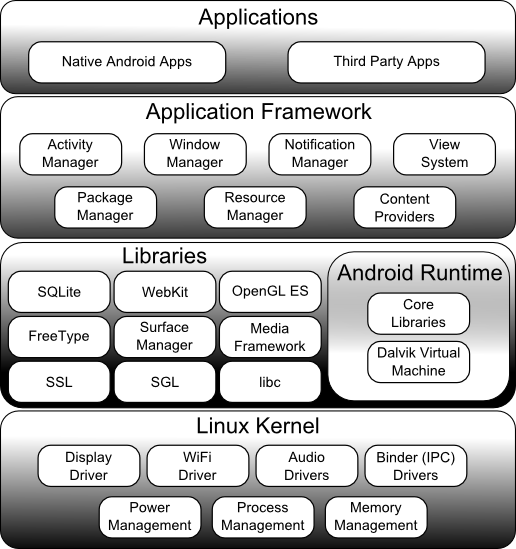
\includegraphics[scale=0.5]{figures/android_architecture.png}
 \end{center}
 \caption{Android architecture}
 \label{fig:android_architecture}
\end{figure}


\subsection{Linux kernel}

Android adopted a famous kernel with proven value concerning efficiency and security. Due to the wide set of constraints that mobile devices present comparing to desktop devices, the Linux kernel suffered some changes. It was properly modified in order to achieve exceptional results in an embedded environment. Therefore, the Android kernel is not a regular distribution of the Linux kernel, but a fork of the mainline kernel source code which allows the Android development team to both implement their necessary changes and follow the Linux kernel updates. This is a big advantage, because the Linux kernel is developed and maintained by a large community that releases, frequently, new patches and versions with enhancements, what lead Android kernel to adopt these enhancements. In fact, every new release of Android usually benefits from a new Linux kernel version. \autoref{tab:android_linux_versions} shows Android releases and the corresponding Linux kernel version.

\begin{table}
\begin{center}
\begin{tabular}{| l | l |}
\hline
\textbf{Android version} & \textbf{Linux kernel version} \\
\hline
Android Cupcake 1.5 & Linux kernel 2.6.27 \\
\hline
Android Donut 1.6 & Linux kernel 2.6.29\\
\hline
Android Éclair 2.0/2.1 & Linux kernel 2.6.29\\
\hline
Android Froyo 2.2 & Linux kernel 2.6.32\\
\hline
Android Gingerbread 2.3.x & Linux kernel 2.6.35\\
\hline
Android Honeycomb 3.x & Linux kernel 2.6.36\\
\hline
Android Ice Cream Sandwich 4.0.x & Linux kernel 3.0.1\\
\hline
Android Jelly Bean 4.1.x & Linux kernel 3.0.31\\
\hline
Android Jelly Bean 4.2.x & Linux kernel 3.4.0\\
\hline
\end{tabular}
\end{center}
\caption{Linux kernel versions and Android realeases}
\label{tab:android_linux_versions}
\end{table}

Google created the \gls{aosp}\footnote{http://source.android.com} to share the Android source code, that goes under the Apache Software License, Version 2.0, and related documentation. Since Android is a product of the Open Set Alliance, which includes a considerable amount of mobile manufactures that present different specifications of hardware, several branches of the Android kernel source code are kept on the git repository\footnote{https://android.googlesource.com}.

The way a mobile device operates is quite different from a laptop or desktop. As mentioned earlier, the Linux kernel suffered several modifications in order to fit a mobile device needs. It became an \textit{Androidized} kernel \cite{EmbeddedAndroid}. The following presents some of the most significant changes and new components brought to the kernel:

\begin{itemize}
 \item \textbf{Wakelocks} was one of the updated components. In Linux, the power management behaves according to the position of the lid in a laptop computer. If the lid is down, the power management will usually put the computer into "suspend" or "sleep" mode, the state of the processes is stored in RAM and the remain hardware turns off. This allows the laptop to save battery power. A mobile device should be in "sleep" mode as often as it is possible, but must not "sleep" when important processes are executing. Wakelocks are used to keep the system awake. Drivers developers need to grab and release wakelocks when important processing is being done or when an application is waiting for the user's input.

 \item \textbf{Low-Memory Killer} executes before the default kernel \gls{oom} killer. When the system lacks of free memory, processes can no longer allocate more memory and the kernel kills a task to get available space. This task is chosen based on priorities. Android's low-memory killer attributes \gls{oom} levels to processes depending on the components they are running and applies a threshold for each type of process. Android avoids the \gls{oom} state by reaching this threshold and killing tasks.

\item \textbf{Binder} is an \gls{ipc} mechanism adopted by Android that was based on OpenBinder. By \gls{ipc} we understand a framework that has the purpose of exchanging signals and data across multiple processes. It is used for message passing, synchronization, shared memory and remote procedure calls. Binder develops an important role among Android application components, as Content Providers, Services, etc \cite{Binder2013}.

\item \textbf{Anonymous Shared Memory (ashmem)} is another \gls{ipc} mechanism that is implemented as the POSIX SHM functionality, part of the System V IPC in Linux. However, the Android development team argued that this mechanism leads to resource leakage within the kernel \cite{EmbeddedAndroid}. Therefore, ashmem is based on POSIX SHM, but takes some enhancements. For instance, it uses reference counting to destroy memory regions when all processes have exited and reduces mapped regions when the system needs memory.

\item \textbf{Alarm} is another example of a driver that required some improvements comparing to the one of the default kernel. Android introduces the alarm timer, an hybrid solution that triggers a \gls{hrt} to fire when an event is supposed to run, while the system is running and, when the system suspends, the alarm timer looks at the list of events  and sets the \gls{rtc} to fire an alarm when the earliest event is to run \cite{AlarmTimer}.

\item \textbf{Logger} is a new mechanism of logging developed specially to Android. In Linux, typically, he find two logging systems: the kernel's own log, accessed through the \texttt{dmesg} command, and the system's log, stored at \texttt{/var/log/}. In Android there is a logger driver on the kernel that maintains circular buffers in RAM where it logs every incoming event \cite{Logger:eLinux}. This contrasts with Linux logging systems, because they use task-switches and file-writers to log each event, turning the process quite complex and heavy.

\end{itemize}

From a security point-of-view, Android inherited the user-based permission model from Linux that will be explained further. A new security feature was implemented on kernel, available as a build option called ANDROID\_PARANOID\_NETWORK, that restricts the access to some networking features, depending on the \gls{gid} of the calling process \cite{AndroidSecurity:AttackAndDefense}.


\subsection{Native Libraries}

Android has a considerable amount of dynamically loaded libraries that supports both Android system to execute internal tasks and  developers to use native code in their applications. Native libraries are written in C/C++, being available through the \gls{jni}. These libraries are placed at \texttt{/system/lib} in the Android filesystem. The following list presents the most relevant libraries:

\begin{itemize}
\item \textbf{Media Libraries} Enables playback and recording of audio and video formats. Based on OpenCore from PacketVideo;
\item \textbf{SQLite} Provides relational databases that can be used by applications and systems;
\item \textbf{SSL} Provides support for typical cryptographic functions;
\item \textbf{Bionic} System C library;
\item \textbf{WebKit} Browser-rendering engine used by Android browsers;
\item \textbf{Surface Manager} Provides support for the display system;
\item \textbf{SGL} Graphics engine used by Android for 2D.
\end{itemize}

\subsection{Android Runtime}

Android development team decided to use Java as the main language to build Android applications, because it is one of the most world wide used programming languages. In Java, there is a Java compiler that translate Java code into architecture-independent byte-code, which is executed at runtime by a byte-code interpreter known as "virtual machine". We are used to the \gls{jvm}. However, it is heavy to mobile devices. Therefore, Google decided to build a new "virtual machine" to deal with Java code and it is called \textit{Dalvik}. Apparently the name was stolen from a village in Iceland. The \gls{dvm} is designed to achieve good results in embedded environments, that uses slow CPUs, less RAM and are battery powered.


\subsection{Application Framework}

Similar to native libraries, the Application Framework offers a set of libraries to support developers. In this layer, libraries are written in Java and are available through Java APIs. The following list describes the most used libraries:

\begin{itemize}
\item \textbf{Activity Manager} Manages the activity lifecycle of applications and various application components. When an application requests to start an activity, Activity Manager provides this service;

\item \textbf{Resource Manager} Provides access to resources such as strings, graphics, and layout files;

\item \textbf{Location Manager} Provides support for location updates (e.g., GPS);

\item \textbf{Notification Manager} Applications interested in getting notified about certain events are provided this service through Notification Manager. For instance, if an application is interested in knowing when a new e-mail has been received, it will use the Notification Manager service;

\item \textbf{Package Manager} The Package Manager service, along with \textit{installd} (package management daemon), is responsible for installing applications on the system and maintaining information about installed applications and their components;

\item \textbf{Content Providers} Enables applications to access data from other applications or share its own data with them;

\item \textbf{Views} Provides a rich set of views that an application can use to display information.

\end{itemize}



\subsection{Applications}

The top layer is composed of the main pieces of the entire system: applications. Android usually comes with several applications, as browser, mail, contacts, etc. Through Google Play, and other third party markets, users may download and install applications that are no different from those previously installed on the device. Android applications present the following filesystem structure:

\begin{itemize}
\item \texttt{src} includes the java packages and files;
\item \texttt{gen} holds auto generated code for resources;
\item \texttt{Android x} contains the android jar file for the targeted version of Android, denoted by \texttt{x} (for instance, \texttt{Android 2.3.3});
\item \texttt{assets} comprises those files that the developer bundles to the application;
\item \texttt{bin} stores files for compiling and running the application, as the \textit{apk} file and \textit{classes.dex} files;
\item \texttt{res} contains all application resources: layouts, values (like strings) and drawables;
\item \texttt{AndroidManifest.xml} defines the application components;
\item \texttt{proguard-project.txt} is the proguard configuration file.
\end{itemize}

Later in this document several references to Android folders will be made.